% Chapter 50: Quantum Theory's Third Route: Path Integrals (Optional)
\chapter[Path Integrals (Optional)]{Quantum Theory's Third Route: Path Integrals (Optional)}

You have seen two quantum outfits: Schrödinger's wavefunctions in Chapter 44, with states evolving continuously, and Heisenberg's matrices in Chapter 46, with observables as tabular operators. They look utterly different yet predict identical digits, suggesting two projections of one deeper structure. This chapter introduces Feynman's third formulation, the path integral. It uses neither wavefunctions nor matrices, only a disarmingly willful idea: count every possible path from start to finish.

This optional chapter can be skipped without affecting later chapters. But it offers two unique rewards: the clearest view of classical mechanics emerging from quantum theory, including Newton, Fermat, and least action; and a principal road to quantum field theory, glimpsed at Chapter 49's end and used for most standard particle-physics calculations today. First declare the level: path integrals are mathematical models and calculation rules, not new experimental facts. Every testable prediction agrees with Schrödinger and Heisenberg. Whenever we say a particle does something, remember that distinction. Our route pins down the double slit's sharpest fact, borrows sound intuition, invents Feynman's arrows, then explains both interference and nature's supposed preference for the easiest route.

\step{A Counterintuitive Opening}

Return to the double-slit apparatus, attending only to experimental facts without theoretical embellishment.

An electron gun sends electrons through two narrow slits onto a screen, each making one bright dot. Reduce the flux until on average at most one electron occupies the apparatus at a time, then wait. Hundreds of dots look disorderly; thousands hint at bands; hundreds of thousands draw crisp, evenly spaced bright and dark stripes, the dark positions completely empty. Laboratories have repeatedly obtained such one-at-a-time interference with electrons, neutrons, and whole molecules.

Now block one slit. Intuition expects half as many electrons and a fainter version of the pattern. Instead the dark bands disappear: positions receiving none among hundreds of thousands now receive electrons steadily.

Side by side, the facts expose the contradiction. At one dark position, slit one alone permits arrival; slit two alone permits arrival; both open forbid it. Each electron passes alone, with no companions to consult; strangers independently vote the pattern into existence. How could one electron know whether the distant slit it never traversed is open?

Hold on to this fact. Every theory must swallow it.

\step{Make a Guess First}

Before new rules, bring your intuitions into the open.

Guess one: does the electron split, half through each slit, then recombine before the screen? Detectors behind each slit should then sometimes catch half an electron. Will they catch halves or whole electrons every time?

Guess two: perhaps blocking a slit brightens dark bands because electrons change routes. Narrow a slit until it barely exceeds the electron's de Broglie wavelength. Does describing a definite thin trajectory through it become easier or harder?

Guess three: mutually exclusive probabilities ordinarily add, one arrival probability through each slit. Dark bands mock that rule. Must we repair probability addition or change what we add? Were the probabilities miscalculated, or were probabilities never the right quantities to sum?

All three answers follow. The third is the key, so here is its spoiler: change the summed object, not probability itself. Quantum mechanics adds probability amplitudes, not probabilities.

\step{Hands-on Experiment}

Though our phenomena are microscopic, path differences determining reinforcement or cancellation can be heard in a living room.

\begin{experiment}[Find Quiet Spots with Two Phones]
Materials: two phones or portable speakers and a single-frequency recording. Search online for a 1 kHz sine wave and play the same file on both phones.

Step one: place the phones side by side on a table, play simultaneously, and walk to the room's opposite end. Set volume just loud enough to hear clearly.

Step two: keeping equal volumes, separate them about a meter, both facing you. Cover one ear and listen with the other while moving slowly parallel to the line joining the phones.

Step three: sound periodically grows louder and softer, nearly silent at minima. Adjacent quiet spots lie about seventeen centimeters apart, half the thirty-four-centimeter wavelength of 1 kHz sound. Measure to check the scale.

Step four: increase speaker separation to two meters and repeat. Quiet spots become more closely spaced. Remember: wider source separation makes finer fringes, exactly the double-slit geometry.

Step five: mute one phone. Quiet spots vanish and sound becomes uniform.
\end{experiment}

Chapters 17 and 18 explain why: unequal paths offset the arriving waves' phase. Differences of whole wavelengths align peaks and troughs, reinforcing sound; a half-wavelength difference makes one push while the other pulls, nearly canceling at your ear. Step five is our opening's acoustic counterpart: turning one source off restores sound where two yielded silence. The same industrious classical-wave mechanism colors soap bubbles and CDs and powers noise-canceling headphones in Chapter 35.

The analogy captures superposition and phase: path differences set phase differences, which set reinforcement or cancellation, with mathematics shared by optical and electron double slits. It differs because sound is real air-density variation, audible and microphone-measurable; the electron's oscillating quantity is an invisible, inaudible probability amplitude, revealed indirectly through probability. Sound cancellation redirects energy rather than destroying it. Quantum dark fringes cancel amplitudes, as we will see.

\step{The Old Model Runs into Trouble}

Lay out the existing theoretical tools and locate each difficulty.

First, probability addition fails. School adds probabilities of mutually exclusive events. Each open slit gives nonzero probability at a dark fringe, but both give zero. Probability theory is not wrong: direct addition requires mutually exclusive, distinguishable events. Without detectors, arrival through slit one and slit two are indistinguishable origins of the same observed screen dot. Indistinguishable origins cannot have their probabilities directly added. This is a rule issue, not arithmetic.

Second, Schrödinger calculates neatly but narrates awkwardly. A wavefunction passes both slits, interferes, and collapses to a dot. That gives the answer without directly explaining why macroscopic objects follow one definite path. A wavefunction fills space; a billiard ball traces a beautiful parabola. Where is the bridge?

Third, classical physics supplies a puzzle. Chapter 13 presented two seeming coincidences: light takes the least-time route, Fermat's principle used for refraction in Chapters 33 and 35; mechanical trajectories make action stationary, the least-action principle used in Chapter 14. Both sound as though nature compares all routes then chooses one. They were useful mathematical facts, but how does nature compare without a computer?

Everyday analogies abound. A lifeguard running faster on sand than swimming in water does not head straight toward a drowning person: the fastest route spends longer on the beach, bending at entry. Air-to-water refraction does the same accounting, its bend minimizing travel time between faster air and slower water. Navigation software likewise estimates totals along routes and ranks the quickest. Each accumulates a quantity along a path and lets the cheapest win. Combine our difficulties: quantum origins all participate, but classically one route survives. A bridge must join these two faces of one phenomenon.

Keep this counterexample handy: intuition says more available routes should improve the chance of arrival. Dark fringes slap it down: two channels add to zero. Our repair must allow adding a positive contribution to reduce the result. Positive-number addition cannot; quantities that change direction can.

\step{Inventing New Concepts}

In the 1940s Feynman took Chapter 13's comparison of all routes seriously, with one reversal: nature does not select one afterward. All enter the account, but most cancel each other. Three rules suffice.

Rule one: assign every possible start-to-finish path a little arrow, all of equal length.

Rule two: action sets each arrow's direction. Action accumulates kinetic minus potential energy over time, as Chapter 14 defined. Each accumulated \(\hbar\), the reduced Planck constant, turns the arrow one full revolution. Large actions spin it rapidly.

Rule three: add all arrows head to tail. The resultant's squared length is proportional to the probability of traveling from start to finish.

These rules had roots. Dirac's 1933 short paper suggested the Lagrangian, kinetic minus potential energy, should matter in quantum theory without specifying how. Feynman developed that hint into a complete theory. His dissertation and 1948 paper made action-dependent phase summation calculable. A hint neglected for fifteen years became quantum mechanics' third route.

\begin{center}
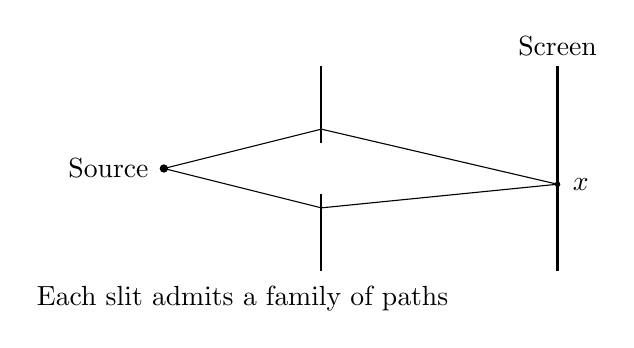
\begin{tikzpicture}[scale=1]
  \fill (0,0) circle (1.5pt) node[left=2pt] {Source};
  \draw[thick] (2,-1.3) -- (2,-0.32);
  \draw[thick] (2,0.32) -- (2,1.3);
  \draw[thick] (5,-1.3) -- (5,1.3) node[above] {Screen};
  \draw (0,0) -- (2,0.5) -- (5,-0.2);
  \draw (0,0) -- (2,-0.5) -- (5,-0.2);
  \fill (5,-0.2) circle (1pt) node[right=2pt] {$x$};
  \node at (1,-1.65) {Each slit admits a family of paths};
\end{tikzpicture}
\end{center}

Declare levels again, as often as needed: these are mathematical rules, not observed processes. No experiment sees an electron actually traverse every path; saying it does exceeds what experiments establish, so this book does not call it fact. Conversely, no experiment supports an undisclosed single definite thin trajectory. What experiments establish is that these calculated probabilities match screen-dot distributions. The theoretical components' private lives in transit remain undisclosed.

Bound the arrow analogy too. Like the speakers, each path supplies a wave contribution, with action playing the role of distance in setting phase. Aligned arrows reinforce and opposite arrows cancel with identical mathematics. But arrows are not spatial vibrations or electron tails, merely pictures of complex numbers, written explicitly in the mathematical bridge. Individual arrows cannot be measured, only probabilities from the squared resultant.

Navigation software offers another comparison. Both schemes assign each route a number accumulated segment by segment: travel time or action. Two differences matter. Navigation discards all but winners; quantum summation retains every path without selecting any. Navigation adds increasing positive quantities, making detours slower; quantum theory adds turning arrows, so detours may enlarge the resultant or annihilate it. These differences hold the answer to the macroscopic single path.

\begin{center}
\begin{tikzpicture}[>=Stealth,scale=0.95]
  \draw[->] (0,0) -- (1,0.07);
  \draw[->] (1,0.07) -- (2,-0.02);
  \draw[->] (2,-0.02) -- (3,0.08);
  \draw[->] (3,0.08) -- (4,0.1);
  \draw[->,very thick] (0,0) -- (4,0.1);
  \node at (2,-1.0) {\shortstack{Near stationarity:\\aligned arrows,\\long resultant}};
  \draw[->] (6.4,0) -- (7.3,0.6);
  \draw[->] (7.3,0.6) -- (7.55,-0.35);
  \draw[->] (7.55,-0.35) -- (8.65,0.1);
  \draw[->] (8.65,0.1) -- (8.25,1.0);
  \draw[->] (8.25,1.0) -- (8.5,0.25);
  \draw[->,very thick] (6.4,0) -- (8.5,0.25);
  \node at (7.5,-1.0) {\shortstack{Far away:\\turning arrows,\\short resultant}};
\end{tikzpicture}
\end{center}

Apply the rules to two slits. Sum all slit-one arrows into \(A_1\), all slit-two arrows into \(A_2\). Total amplitude is \(A_1+A_2\). At dark fringes, \(A_1\) and \(A_2\) have equal lengths and opposite directions, summing to zero. Individually passable routes produce darkness together. Arrow addition succeeds where probability addition fails.

\step{The Model in One Sentence}

\begin{oneline}
Give every possible start-to-finish path an equal-length arrow directed by its action, turning one full revolution per \(\hbar\), then add them all; the resultant's squared length gives probability. Classical paths are special not because they are selected, but because neighboring arrows nearly align instead of canceling.
\end{oneline}

This joins quantum all-path accounting and the conspicuous classical single path: not separate worlds, but one rule at two scales of accounts.

\step{The Mathematical Translator}

Recall Chapter 14's action:
\[
S=\int L\,\mathrm{d}t,\qquad L=T-V,
\]
kinetic minus potential energy accumulated over time. Translate the three arrows into a formula. Each path contributes amplitude proportional to
\[
\mathrm{e}^{\mathrm{i}S/\hbar},
\]
a complex number of length \(1\) and angle \(S/\hbar\), precisely an arrow. Summing all contributions gives
\[
K=\sum_{\text{all paths}}\mathrm{e}^{\mathrm{i}S/\hbar},
\qquad\text{probability}\propto |K|^2 .
\]

As always, test special cases first.

Check one: only two paths, with \(S_1=S_2\). Arrows align, doubling resultant length and multiplying probability by \(4\), not \(2\). Adding amplitudes before squaring produces interference terms; bright fringes exceed simply added slit probabilities. The formula passes.

Check two: \(S_1-S_2=\pi\hbar\), half a turn between arrows. They cancel, leaving zero amplitude and probability. Two nonzero contributions yield zero: scandalous for ordinary probabilities, straightforward here. This is a dark fringe, another passed check.

Check three: let \(\hbar\) approach zero, or equivalently make action much larger than \(\hbar\). Tiny path deviations send \(S/\hbar\) through thousands of revolutions, and neighboring arrows cancel. Only stationary paths escape: first-order changes in action vanish nearby, so a small cluster aligns, survives collectively, and makes a long resultant. Chapter 13's least-action principle emerges not as an independent law but as the \(S\gg\hbar\) approximation to summation. Correct the historical phrasing: stationary, not minimum, is essential, resolving Chapter 13's earlier hint.

Keep the geometry: fix endpoints and draw straight, curved, and winding candidate paths. A small cluster around a stationary path gives aligned arrows and a long resultant; farther away, neighboring action differences grow, arrows scramble, and the sum shrinks. Only a narrow tube around stationarity substantially contributes, its width determined by \(\hbar\) relative to action. An electron's tube is roughly its de Broglie wavelength wide, allowing two through a double slit; a billiard ball's is unimaginably thin, leaving one apparent macroscopic route.

\begin{center}
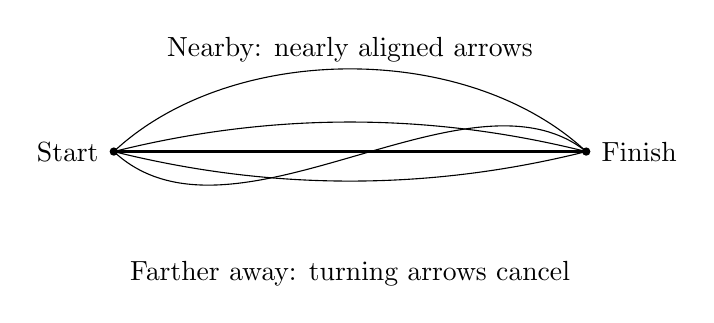
\begin{tikzpicture}[scale=1]
  \fill (0,0) circle (1.5pt) node[left=2pt] {Start};
  \fill (6,0) circle (1.5pt) node[right=2pt] {Finish};
  \draw[very thick] (0,0) -- (6,0);
  \draw (0,0) .. controls (2,0.5) and (4,0.5) .. (6,0);
  \draw (0,0) .. controls (2,-0.5) and (4,-0.5) .. (6,0);
  \draw (0,0) .. controls (1.5,1.4) and (4.5,1.4) .. (6,0);
  \draw (0,0) .. controls (1.5,-1.4) and (4.5,1.2) .. (6,0);
  \node at (3,1.3) {Nearby: nearly aligned arrows};
  \node at (3,-1.55) {Farther away: turning arrows cancel};
\end{tikzpicture}
\end{center}

\begin{mathbridge}
Why stationary paths survive can be more precise. Let parameter \(a\) deform a family of curves, making action an ordinary function \(S(a)\). Phase \(S(a)/\hbar\) varies with \(a\) at rate \(S'(a)/\hbar\). Small \(\hbar\) makes tiny parameter changes produce many phase turns, so opposite arrows cancel. Only near \(S'(a)=0\) does the rate cross zero, leaving nearly constant phase over a substantial parameter interval and coherent contributions. This stationary-phase approximation is a precise accessible meaning of classical mechanics as a quantum approximation.

Amplitudes also compose elegantly: travel from A to C through an intermediate time equals the sum over all intermediate positions B of the A-to-B amplitude times the B-to-C amplitude. Multiplication relays arrows by adding angles, reflecting additive action; summation admits any intermediate location. Repeating this law while slicing time infinitely finely defines the path integral rigorously, akin to ordinary integration's small-slice sums, but now summing curves themselves rather than area beneath one curve.
\end{mathbridge}

Estimate real scales to locate the border between microscopic many-path and macroscopic single-path behavior.

Start with a 100 eV electron, a typical electron-microscope scale. Its de Broglie wavelength is about \(1.2\times10^{-10}\) m and speed \(6\times10^{6}\) m/s. Over one meter, action is kinetic energy times duration, \(S\sim 1.6\times10^{-17}\times1.7\times10^{-7}\approx3\times10^{-24}\) J·s, so \(S/\hbar\approx3\times10^{10}\). Astronomical, but not hopeless: differences depend on path-length differences, and a \(\pi\) phase difference requires half a wavelength, about \(6\times10^{-11}\) m, smaller than an atom. Micrometer slit separation yields roughly \(10^{-4}\) m screen fringes, readily measurable with magnification. Electrons enjoy multiple-path coherence.

Now a sand grain: mass \(10^{-6}\) kg, speed 1 m/s, distance one meter. Action is about \(5\times10^{-7}\) J·s, hence \(S/\hbar\approx5\times10^{27}\). Interference would require slit spacing comparable to its roughly \(7\times10^{-28}\) m de Broglie wavelength, over a dozen orders below a proton's diameter, utterly unfabricable. A macroscopic deviation of one hundred-quintillionth of a meter already spins arrows through countless turns, canceling completely. Classical paths are not nature's choice but the sole survivors of summation's civil war.

\begin{challenge}
Why do path sums reproduce Schrödinger? Feynman's original paper divides time into \(N\) tiny intervals, approximates each segment as straight, and turns path summation into the limit of \(N\)-fold ordinary integrals. One can then prove the amplitude evolves by Schrödinger's equation. Another profound move replaces time by imaginary time \(\tau=\mathrm{i}t\), turning \(\mathrm{e}^{\mathrm{i}S/\hbar}\) into decaying weight \(\mathrm{e}^{-S_E/\hbar}\). Violent cancellation becomes gentle weighting, resembling Chapter 31's statistical partition function: quantum and statistical mechanics are close mathematical relatives. This underlies modern field-theory calculations. Supercomputers sample field configurations with these weights in lattice quantum chromodynamics, predicting proton mass from first principles to about one percent agreement. Expanding interactions order by order produces networks of vertices and lines, Feynman diagrams, whose sketches of particle creation and annihilation appeared in Chapter 49.
\end{challenge}

\step{The Model's Limits}

Powerful path integrals need five boundaries.

First, exact equivalence is not new physics. Every testable nonrelativistic point-particle question gives identical path-integral, Schrödinger, and Heisenberg predictions. These are three accounts of one model, chosen for convenience: path integrals often simplify scattering and field quantization; Schrödinger more directly solves Chapter 52's hydrogen levels. None is more real.

Second, paths are not travel diaries. Each is a summation index, like integration's little rectangles, a calculation component. Identifying one with the electron's actual journey confuses mathematics and observation, the same discipline that kept Chapter 43 from drawing definite-orbit electron balls.

Third, which-path information changes the rule. Once apparatus makes paths distinguishable in principle, even if nobody reads stored data, probability replaces amplitude addition and fringes disappear. This is not crude instruments battering electrons: arbitrarily small disturbance still destroys interference if paths become distinguishable. The reason lies in quantum addition, not manufacturing quality.

Fourth, measurement remains unsolved. Reformulating quantum theory does not explain why this trial lands at this dot. Like wavefunctions, path integrals supply probabilities and no more. Decoherence explains lost fringes in open systems without resolving the entire measurement problem, equally in all three languages.

Fifth, the framework has limits. Here we sum paths of one fixed particle. Chapter 49's changing high-energy particle count requires sums over all field configurations instead. Converting Lagrangian path language to Hamiltonian state language also requires conditions; a Hamiltonian is not unconditionally total energy, as Chapter 15 cautioned.

Finally reject a fashionable misuse: all paths means anything is possible. Bizarre paths, even circling the Moon before reaching the screen, enter the account, but their arrows almost entirely cancel into indescribably tiny contributions. Being recorded and producing observable consequences are separated by destructive interference. Path integrals broaden calculation's scope, not the quota of miracles.

\step{Explaining the Opening Phenomenon}

Settle the opening paradox item by item.

Why no dots in dark fringes? Slit-one paths sum to \(A_1\), slit-two paths to \(A_2\), and there \(A_1\) and \(A_2\) are equal and opposite. Total amplitude and probability vanish.

Why does blocking one slit restore arrivals? It removes the entire \(A_2\) family, leaving \(A_1\) with nonzero probability. Electrons neither split, consult, nor sense the other slit. The amplitude sum's domain changes. Different apparatus defines different events and hence distributions; the strange part is our attachment to direct probability addition.

Fringe geometry follows too. Moving from dark to neighboring bright changes the action difference by \(\pi\hbar\), a half de Broglie wavelength of path difference. Greater slit separation produces the same path difference over a smaller screen displacement, giving finer fringes, just as wider speaker spacing tightened quiet spots in step four. Sound, light, and electrons share one geometry, with different turning quantities: sound pressure, electric field, and probability amplitude.

Answer the guesses. First, detectors always catch whole electrons, never halves, but distinguishing paths destroys fringes. Second, narrower slits localize passage more precisely and increase transverse momentum uncertainty, spreading fringes wider; a definite thin line becomes harder, fundamentally rather than instrumentally. Third, add amplitudes, not probabilities directly. Amplitudes can be positive, negative, and change direction, making a reduced sum after adding a contribution ordinary rather than paradoxical.

A quieter reward retires Chapter 13's anthropomorphic easiest-route language. Nature neither compares nor chooses: every path votes, but macroscopically only near-stationary votes align and the rest cancel. Least action is a statistical result, not a legislative decree.

\step{Thought Experiments and Challenges}

\begin{thought}[Infinitely Many Slits]
Open three slits and add three path families; ten, a thousand, enough to perforate the barrier completely, then remove it. The same logic makes free propagation a sum over every free-space path. This is the path integral's original inspiration, not mathematical acrobatics. Double slits reduce the general rule to two families; barriers merely delete summation terms.

Push the scale: suppose \(\hbar\) were not \(10^{-34}\) J·s but 1 J·s. A billiard ball's action would be a few \(\hbar\), and deviations from straight paths would no longer cancel cleanly. Crossing the table, the ball would spread into a probability cloud and form fringes behind a double-slit barrier. The lesson: quantum/classical boundaries depend on action relative to \(\hbar\), not size. Large objects are classical because their accounts make \(\hbar\) so tiny that path disagreements immediately cancel.
\end{thought}

Where next? Replace path sums with field sums to obtain the standard field theory behind Chapter 49's ending. Sum over spacetime geometries themselves and enter quantum-gravity research marked on Chapter 61's map. A rule born at two slits reaches physics' frontier construction site.

Close with the book's three questions. What is the present state? Path integrals change viewpoint, not the answer: ask not where a particle is now, but the amplitude from an initial state to every possible outcome, summing all path arrows. What governs change? Action, assigning phases as the sole legislator, with classical mechanics its approximate silhouette. How does measurement reveal it? Still only through probabilities, squared resultant lengths, one dot per trial and accumulated fringes. Three languages, one answer sheet: powerful evidence of one underlying reality.

\begin{puzzles}
\item Replace two slits with three. Must an original dark-fringe position remain dark with all three open? (Hint: all resultant arrows must sum to zero. Two equal arrows cancel only oppositely; three need only form a closed triangle head to tail, a less restrictive condition.)
\item Put very thin glass behind slit one. Passage slightly changes electron action, rotating \(A_1\) while leaving \(A_2\) unchanged. What happens to fringes? (Hint: darkness depends on relative angle. Alter it and equal-and-opposite positions move: the whole pattern shifts, retaining bright/dark spacing. This is indeed a standard experimental fringe-shifting method.)
\item If all paths count, why do the two slit families suffice? What about paths hitting the barrier? (Hint: candidates must reach the chosen screen point from the source. Absorbed paths cannot, so are excluded. Changing the barrier changes the event definition and summation domain, the arithmetic reason blocking changes probability.)
\item For a \(10^{-6}\) kg sand grain moving at 1 m/s, what slit-spacing scale would show interference? (Hint: fringes depend on \(\lambda=h/(mv)\). Estimate it and ask whether such slits can be fabricated: this quantifies the macroscopic single path.)
\end{puzzles}
